\subsection{DCGAN}
\label{sec:exp-dcgan}

We implement our baseline model in this section. The DCGAN is evaluated on cifar10. We present the evolution of the inception score in Figure \ref{fig:exp-dcgan-is} and both losses in Figure \ref{fig:exp-dcgan-losses}
   
\begin{figure}[h]
\centering
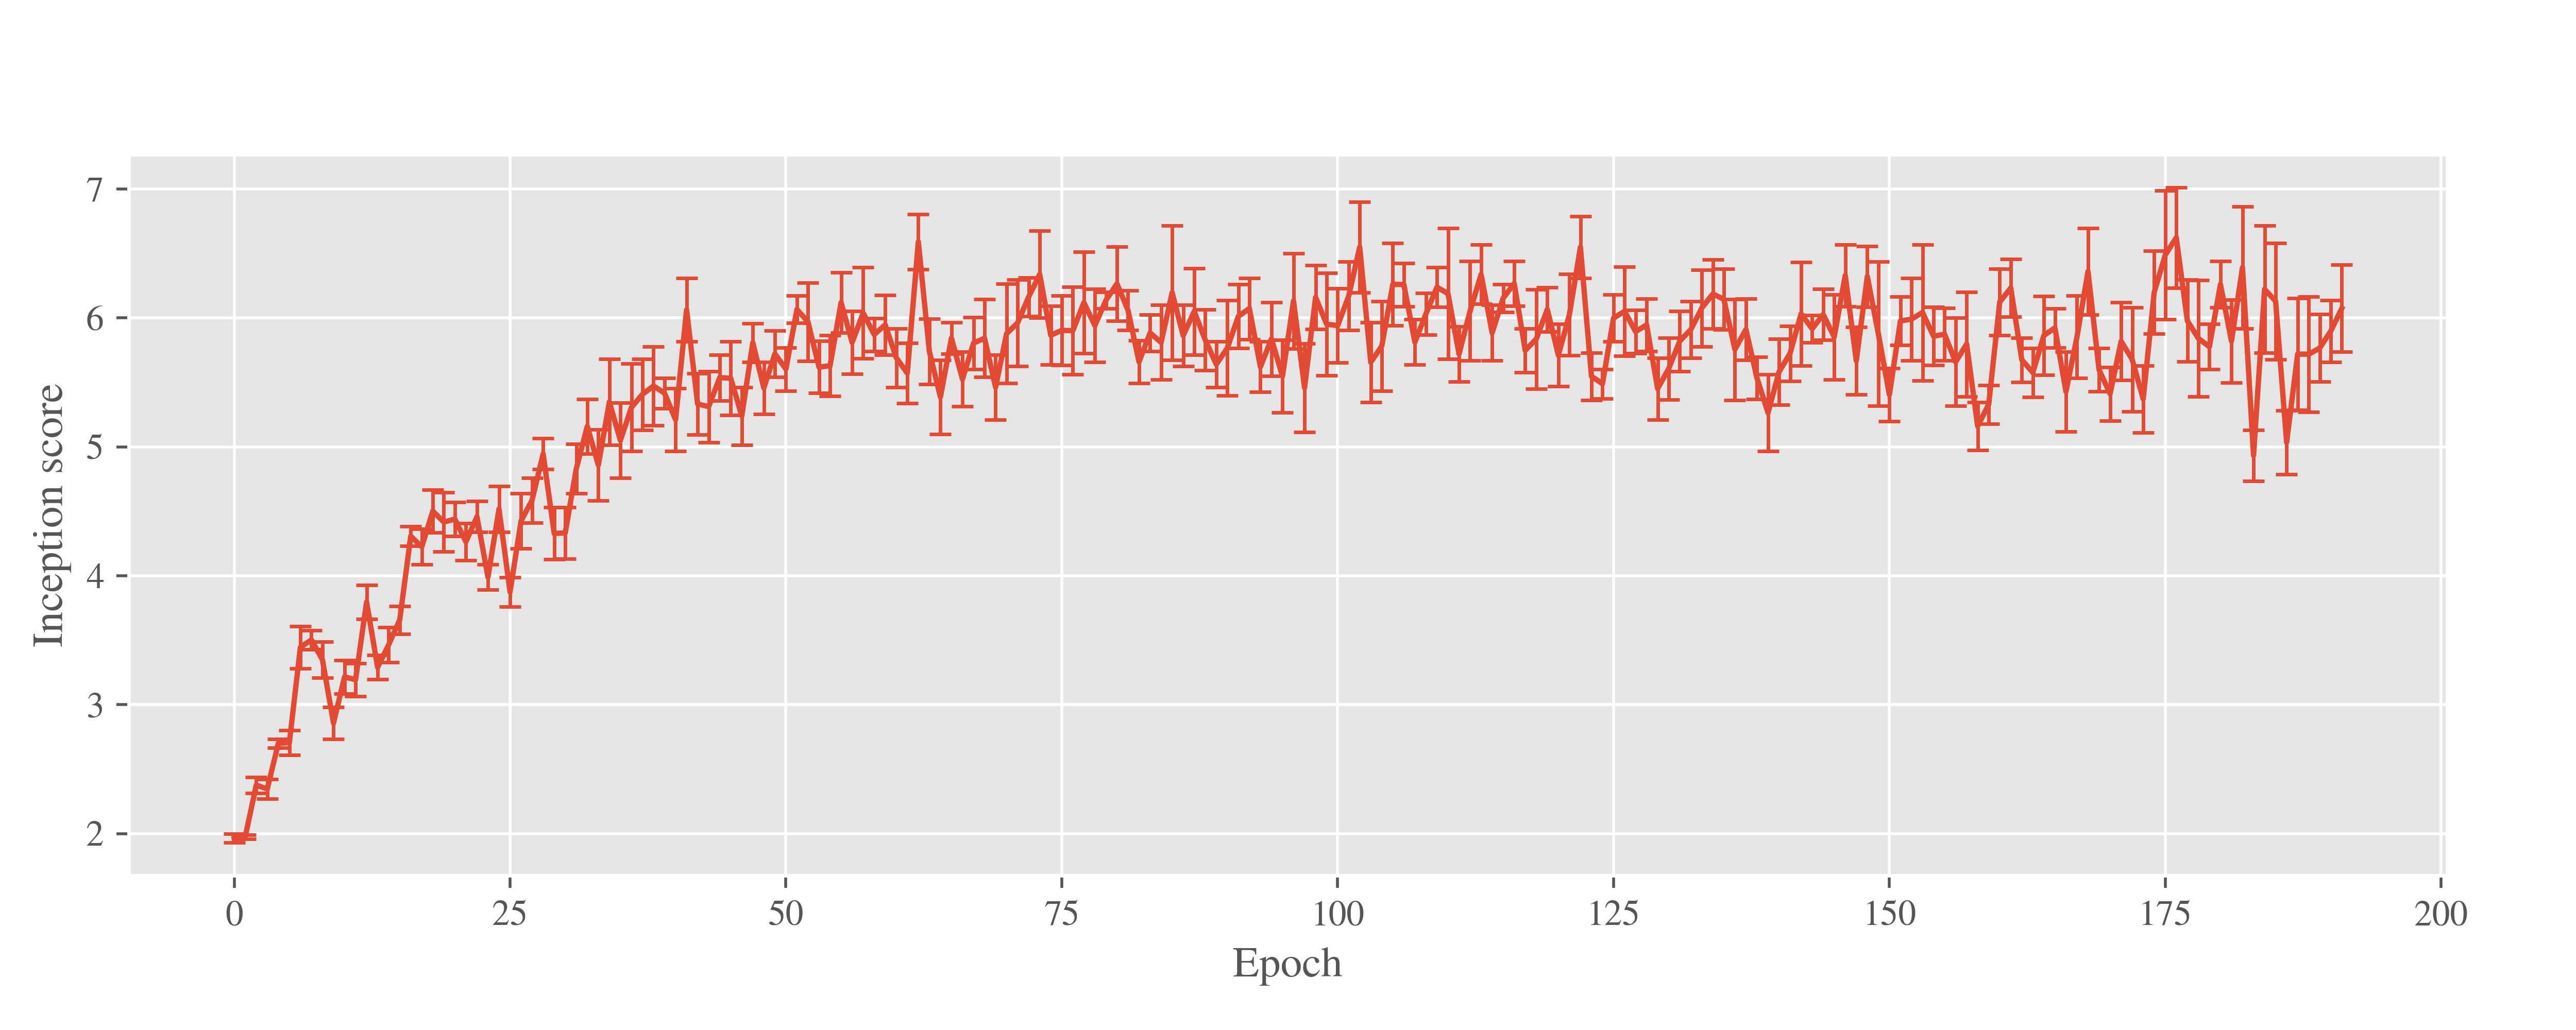
\includegraphics[width=\textwidth]{../code/results/figures/dcgan_cifar10_is.png}
\caption{DCGAN - Inception score, training on cifar10 over 190 epochs}
\label{fig:exp-dcgan-is}
\end{figure}


\begin{figure}[h]
\centering
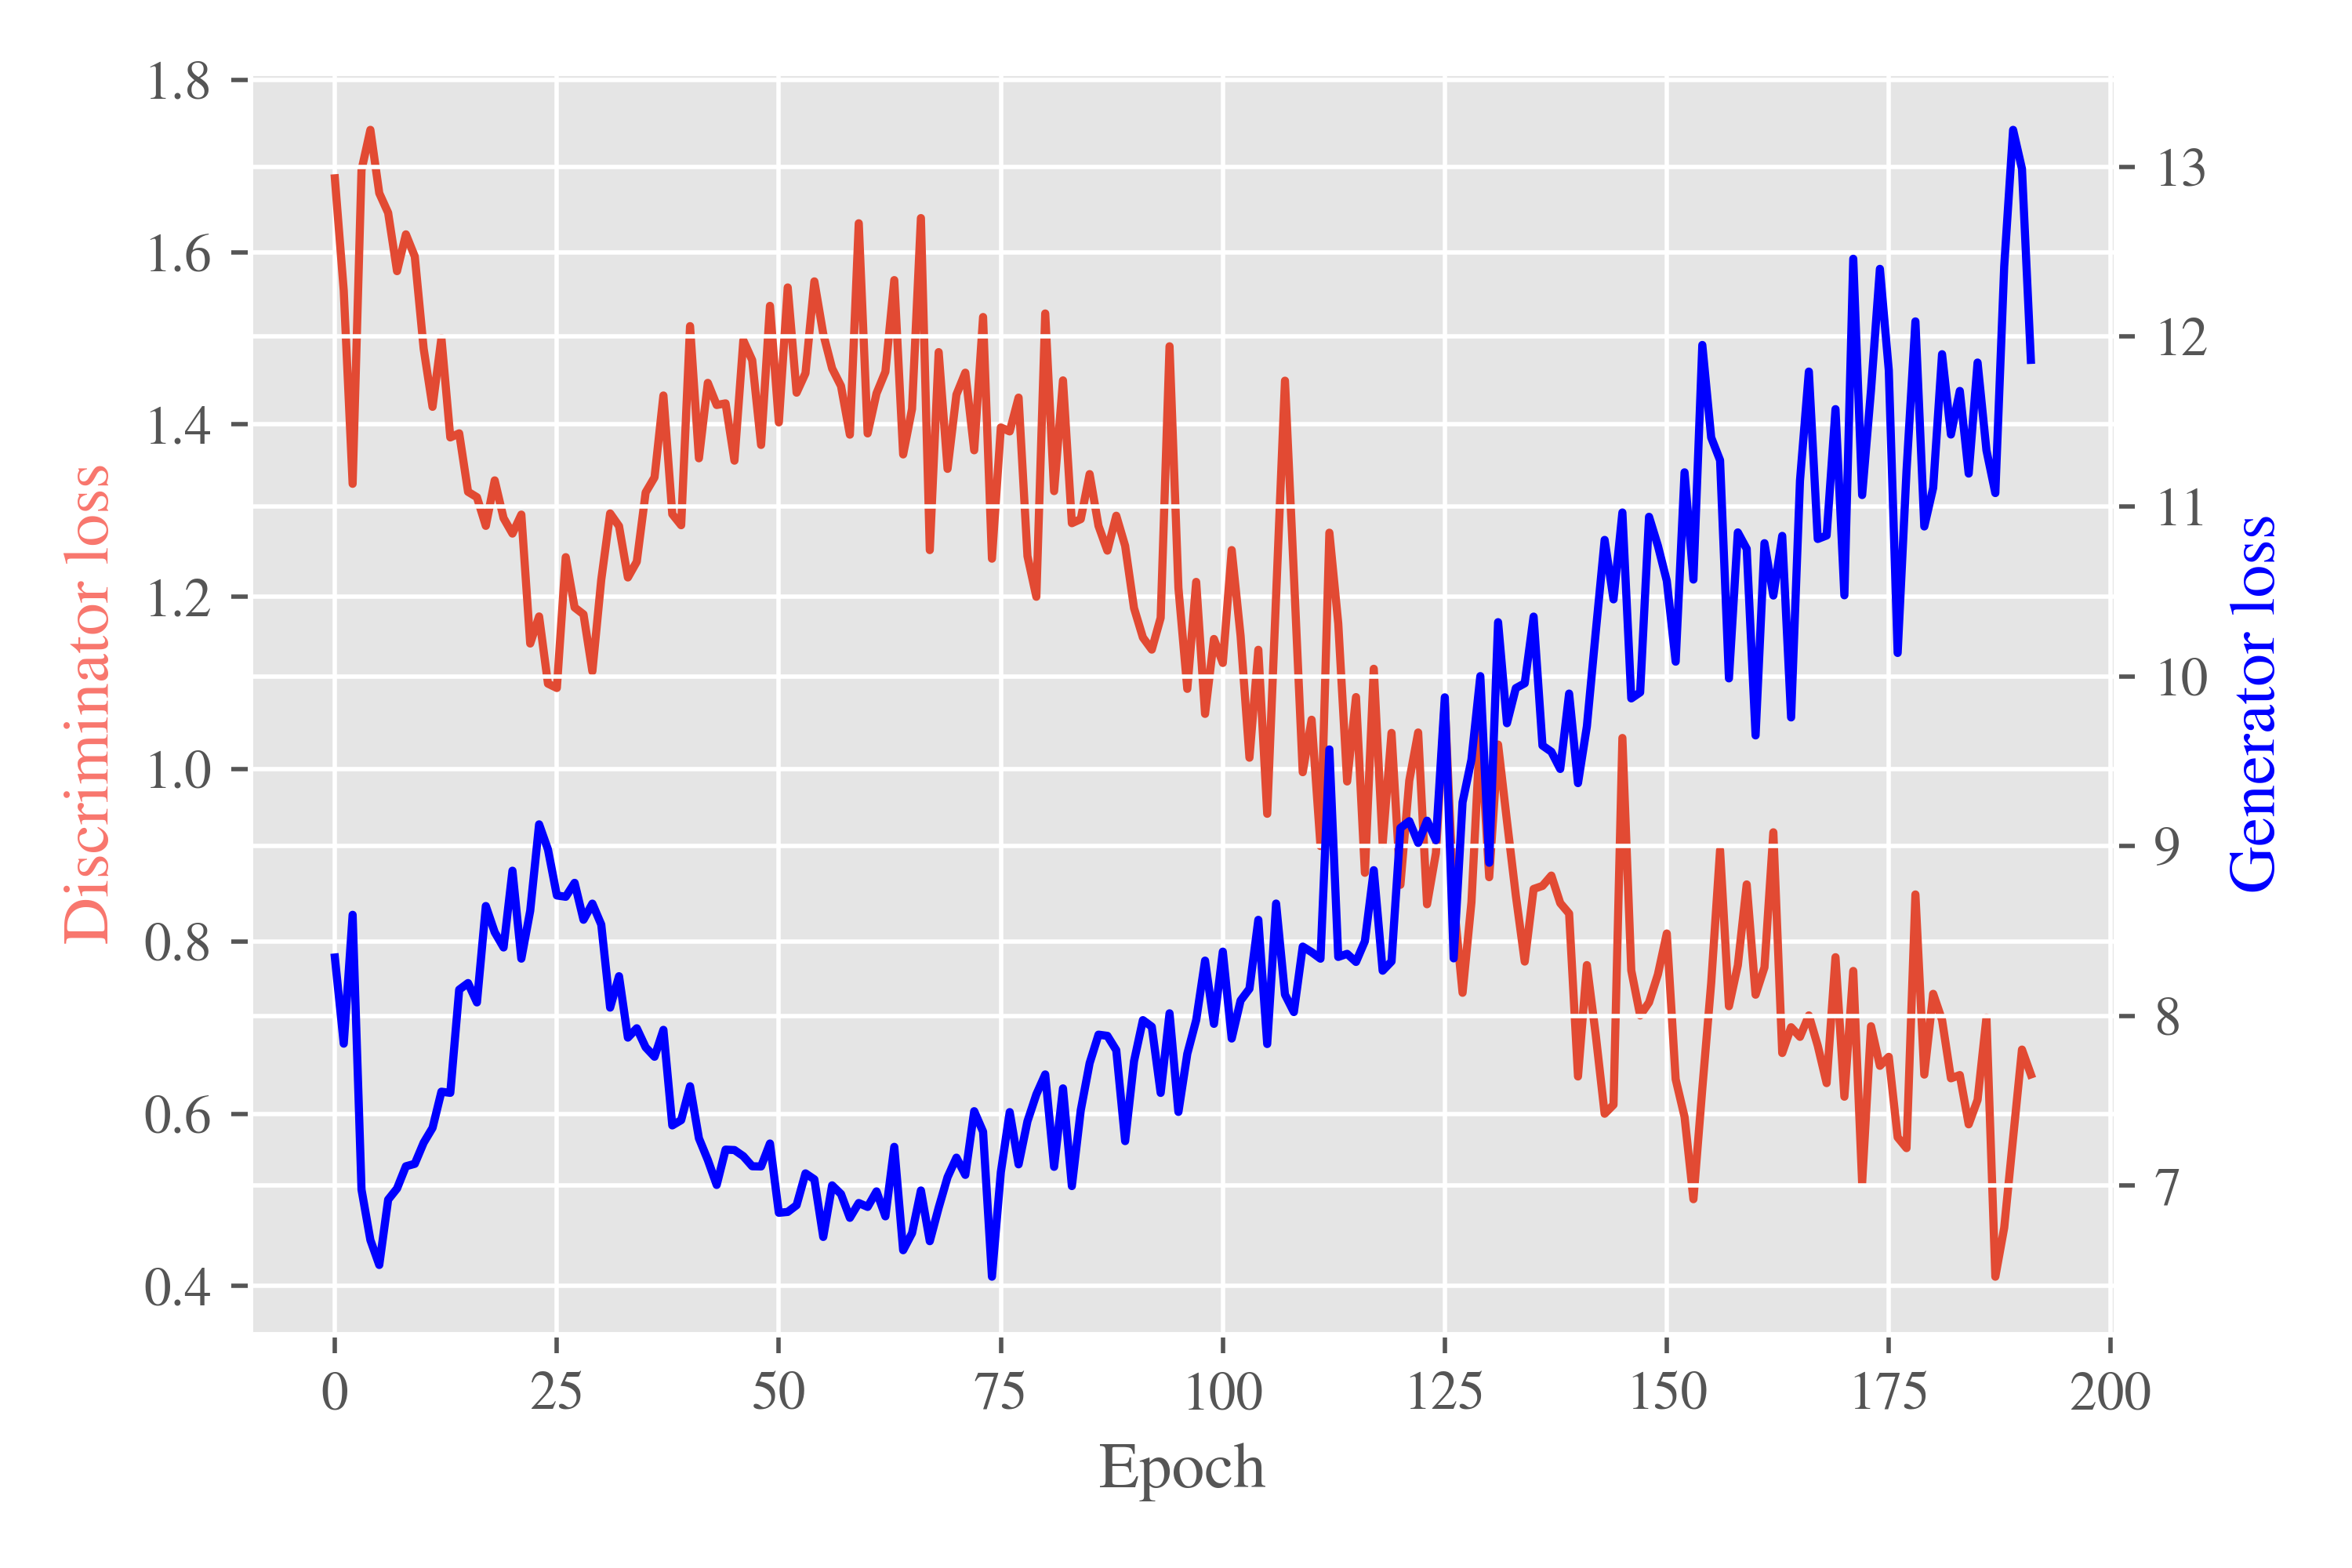
\includegraphics[width=\textwidth]{../code/results/figures/dcgan_cifar10_losses.png}
\caption{DCGAN - Losses training on cifar10 over 190 epochs.}
\label{fig:exp-dcgan-losses}
\end{figure}

Losses can hardly be interpreted when treating with GANs, since the generator and discriminator are in a situation of competition where an improvement on the one leads to a deterioration on the other.

